\documentclass[conference]{IEEEtran}
% The preceding line is only needed to identify funding in the first footnote. If that is unneeded, please comment it out.
\usepackage{cite}
\usepackage{amsmath,amssymb,amsfonts}
\usepackage{algorithmic}
\usepackage{graphicx}
\usepackage{textcomp}
\usepackage{xcolor}
\def\BibTeX{{\rm B\kern-.05em{\sc i\kern-.025em b}\kern-.08em
    T\kern-.1667em\lower.7ex\hbox{E}\kern-.125emX}}
\begin{document}

\title{Immersivaudio: audio generation based on video features.\\
{\footnotesize Group 01}
}


\author{\IEEEauthorblockN{Michele Vitale}
\IEEEauthorblockA{\textit{ist1111558}}
\and
\IEEEauthorblockN{Daniele Avolio}
\IEEEauthorblockA{\textit{ist1111559}}
\and
\IEEEauthorblockN{Teodor Chakarov}
\IEEEauthorblockA{\textit{ist1111601}}
}

\maketitle


\begin{IEEEkeywords}
component, formatting, style, styling, insert
\end{IEEEkeywords}

\section{Introduction}
The topic of media generation has been exponentially growing during the last few years. Since the release of models and services based on state-of-art AI techniques, such as StableDiffusion and ChatGPT, it has been frequent to have media generative applications, with the most important part being that they can be easily accessed even by users that do not have competences and knowledge on Artificial Intelligence. 
Our proposal is a pipeline composed of different models, trained or open-wheigths, to generate audiovisive multimedia. 

\section{Problem description}
Main goal of our project is to provide a tool capable of enhance the audio track of an input video, by extracting main features such as objects, environment or tone. The tool should be easy to deploy, modular, without any particular knowledge previously required to the user, intuitive. After further research on and state-of-art models, we might extend the project to generate also music. The feasibility of that, with a good quality of the outcome, will require some test at later stage, with a first part of the implementation already deployed. Further features will be implemented during the development of the project, coming out from the useful options that we might see during the development stages. 


\section{Problem importance}
The problem can have a practical use in those cases in which the audio track of a video is not enjoyable, or not present at all. For instance, we can think about recordings made from drones or submarine cameras. If deployed in an accessible shape, like a very simple application, the tool can be also used by visually impaired people that can get a more immersive experience from a video or from the environment surrounding them. 
Last but not least, it might result useful for content creators that need to publish their videos on platforms that have strict Copyright policies, such as YouTube. The tool could be helpful by producing some copyright-free audio track without having to rely on Copyright-free music, that might require time to be incorporated in the video track and might be already used by other creators.

\section{Architecture}
The complete architecture will be extended on four main modules, that will be connected as shown in the picture. The modules will be pluggable in a way that every single one, apart from reconstructor which is very related to the complete process, can be used as standalone parts, as long as the input shape is respected.\\
It is important to note that this is a first draft of the final architectures, so changes might apply at development stage.

\begin{figure}
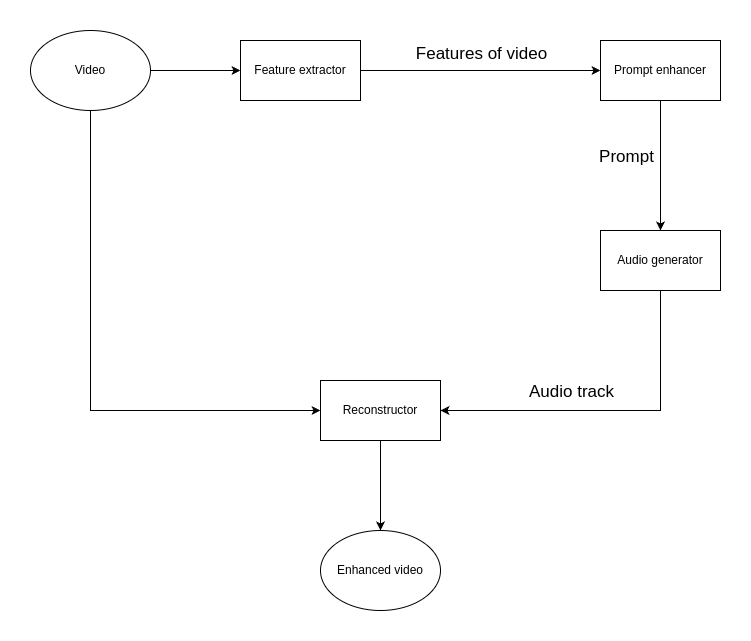
\includegraphics[width=\linewidth]{architecture.drawio.png}
\caption{Architecture schema}
\end{figure}


\subsection{Feature extraction}
The feature extraction module takes an input video, in most common video extensions, and processes it to extract relevant features such as present objects, context etc.\\
The expected output will be a list of keywords that can explain the context of the video, as well as the main subjects present. On that stage, we will rely on Yolo and OpenCV (temporary, will add references).
\subsection{Prompt enhancer}
The prompt enhancer will get as input the list of features produced by the first module. The expected output will be a complete and organized prompt that will be fed to the following module. This model might be either composed by a simple string interpolated with the extracted keywords or a Large Language Model locally deployed. Components of this module will be defined with further tests on the audio generation model, to first understand what fits better for it. 
\subsection{Audio generator}
The audio generation part will be taking as input the conditional prompt, giving in output the audio track that will be combined to the video. This part will rely on audiociosioeiroeireor insert reference here, with further tests conducted in the music generation direction. 
\subsection{Reconstructor}
This module will take both the input video and the audio track in output from the previous module, as well as eventual input parameters provided by the user. It will combine the track to the video using FFMPEG, then it return the result of the complete process to the user. 

\section{Possible features}
output format, output type (song or video+song), music or audio option etc 
\section*{References}

REFERENCES STILL TO BE PUT HERE
\begin{thebibliography}{00}
\bibitem{b1} G. Eason, B. Noble, and I. N. Sneddon, ``On certain integrals of Lipschitz-Hankel type involving products of Bessel functions,'' Phil. Trans. Roy. Soc. London, vol. A247, pp. 529--551, April 1955.
\end{thebibliography}
\end{document}
